\documentclass[nometaot,lecture,amberg,toc=twocolumn,indicatelastpageofframe,footlinebox]{OTHAWbeamer}

% Packages
\usepackage{graphicx}
\usepackage{animate}
\usepackage{booktabs}
\usepackage{amsmath}
\usepackage{tikz}
\usepackage{multicol}
\usepackage{array}
\usepackage{caption}
\usepackage{subcaption}
\usepackage{colortbl}
\usepackage{svg}

\usetikzlibrary{positioning, arrows.meta, shapes.geometric}

% Pre-defined tint colors to avoid xcolor conflicts inside Beamer frames
\colorlet{lila1light}{lila1!10}
\colorlet{lila1med}{lila1!12}
\colorlet{blau1light}{blau1!10}
\colorlet{cyan1light}{cyan1!10}
\colorlet{cyan1vlight}{cyan1!8}
\colorlet{cyan1med}{cyan1!15}
\colorlet{gruen1light}{gruen1!10}


\graphicspath{{images/}}

% Presentation Information
\title{IN-CONTEXT CASCADE SEGMENTATION}
\subtitle{AI-Conference}

\author{Hemanthkumar Muthusamy Gunasekaran}
\institution{Ostbayerische Technische Hochschule Amberg-Weiden}

\place{Amberg}
\date{\today}

\email{h.muthusamy-gunasekaran@oth-aw.de}

\def\inserttoctitle{Overview}


%\includeonlyframes{current}

% ============================================================
\begin{document}
% ============================================================

% Title Page
\setbeamerfont{title}{size=\LARGE}
\maketitle
\setbeamerfont{title}{size=\huge}

% Table of Contents
\begin{frame}{Overview}
    \begin{columns}[t]
        \column{0.5\textwidth}
            \tableofcontents[sections={1-3},hideallsubsections]
        \column{0.5\textwidth}
            \tableofcontents[sections={4-6},hideallsubsections]
    \end{columns}
\end{frame}

\section{Introduction}
\begin{breakframe}
    Introduction
\end{breakframe}
% ============================================================
% SECTION 1 — INTRODUCTION
% ============================================================

% --- Slide 0 ---
\subsection{From Scanner to Slice}
\begin{frame}
    \frametitle{How MRI and CT work}
    \framesubtitle{Before we start}

    \begin{columns}[t]

        \column{0.50\textwidth}
            MRI and CT scanners generate \textcolor{orange1}{\textbf{3D volumes}}
            by capturing sequential 2D cross-sectional slices of patient anatomy.

            \vspace{0.6em}

            \vspace{0.6em}

            \begin{block}{Scope of This Work}
                Here we use only \textbf{sequence of 2D slices}
                avoiding the computational cost of full 3D model training.
            \end{block}

        \column{0.47\textwidth}
            \vspace{0pt}
            \centering
            \includesvg[width=\linewidth, height=0.6\textheight, keepaspectratio]{Intro}

            \vspace{0.3em}
            {\tiny\textcolor{grau2}{Source: \href{https://www.mayoclinic.org/tests-procedures/ct-scan/multimedia/ct-scan-slices/img-20008348}{Mayo Clinic CT Scan Slices}}}

    \end{columns}

\end{frame}

% --- Slide 1 ---
\subsection{The Problem}
\begin{frame}
    \frametitle{The Problem}
    \framesubtitle{Where It All Starts}

    \begin{columns}[c]

        \column{0.55\textwidth}

            Manual annotation of \textcolor{orange1}{\textbf{hundreds of slices}}
            per patient is a time-consuming bottleneck for radiologists.

            \vspace{0.6em}
            The huge volume of annual hospital scans makes this manual approach
            \textcolor{orange1}{\textbf{impossible to sustain}}.

            \vspace{0.6em}
            Current models lack diversity forcing a \textcolor{orange1}{\textbf{complete restart}}
            whenever imaging modalities or target organs change.\textsuperscript{[1,2]}

    

        \column{0.42\textwidth}
            \centering
            \begin{tikzpicture}[scale=0.85]
                % MRI slice stack
                \foreach \i in {0,1,2,3,4} {
                    \draw[fill=grau4, draw=grau2, rounded corners=1pt]
                        (0.12*\i, 0.18*\i) rectangle ++(2.6, 1.5);
                }
                % top slice highlight
                \draw[fill=cyan1med, draw=cyan1, rounded corners=1pt, line width=0.8pt]
                    (0.48, 0.72) rectangle ++(2.6, 1.5);
                \node[font=\tiny, text=grau1] at (1.78, 1.47) {slice $k$};

                % annotation pen icon
                \draw[orange1, line width=1.2pt, -{Stealth[length=4pt]}]
                    (3.3, 1.8) -- (2.5, 1.3);
                \node[font=\scriptsize, text=orange1, anchor=west] at (3.35, 1.85)
                    {\textbf{annotate}};

                % clock
                \draw[grau1, line width=0.8pt] (1.78, -0.7) circle (0.45);
                \draw[grau1, line width=0.8pt] (1.78, -0.7) -- (1.78, -0.38);
                \draw[grau1, line width=0.8pt] (1.78, -0.7) -- (2.03, -0.7);
                \node[font=\tiny, text=grau1] at (1.78, -1.28) {hours per scan};

                % scale label
                \node[font=\scriptsize\bfseries, text=orange1] at (1.78, -1.75)
                    {$\times\,1000$ scans each year};
            \end{tikzpicture}

    \end{columns}

\end{frame}

% --- Slide 2 ---
\subsection{The Need for Segmentation}
\begin{frame}
    \frametitle{The Need for Segmentation}
    \framesubtitle{Why Automating Medical Image Analysis Matters}

    AI research in healthcare has grown rapidly driven by significant
    progress in \textcolor{orange1}{\textbf{deep learning}} techniques.

    \vspace{0.8em}

    Automating the segmentation of CT and MRI sequences is vital for
    \textcolor{orange1}{\textbf{surgical planning}},
    \textcolor{orange1}{\textbf{radiotherapy}}, and
    \textcolor{orange1}{\textbf{monitoring cancer treatment}}.

    \vspace{0.8em}

    The high costs and manual labor involved in these tasks create an
    urgent demand for \textcolor{orange1}{\textbf{automated solutions}}.

\end{frame}

% --- Slide 3 ---
\subsection{Evolution of Deep Learning in Segmentation}
\begin{frame}
    \frametitle{Evolution of Deep Learning}
    \framesubtitle{From U-Net to Foundation Models}

    \centering
    \begin{tikzpicture}

        % horizontal backbone
        \draw[line width=2.5pt, orange1, -{Stealth[length=7pt]}] (-0.3,0) -- (11.8,0);

        % ---- U-Net ----
        \draw[fill=lila1, draw=lila1] (1.2,0) circle (6pt);
        \draw[lila1, line width=1pt] (1.2,0) -- (1.2,1.1);
        \node[draw=lila1, fill=lila1, rounded corners=4pt, minimum width=3.8cm,
              minimum height=1.1cm, align=center, font=\small, text=weiss, anchor=south]
              at (1.2,1.1) {\textbf{U-Net}\\[2pt]{\tiny Encoder-decoder + skip connections}};
        \node[draw=lila1, fill=lila1, rounded corners=2pt, minimum width=1cm,
              minimum height=0.42cm, font=\tiny\bfseries, text=weiss, anchor=north]
              at (1.2,-0.35) {2015};

        % ---- ViT / Swin ----
        \draw[fill=blau1, draw=blau1] (4.2,0) circle (6pt);
        \draw[blau1, line width=1pt] (4.2,0) -- (4.2,-1.1);
        \node[draw=blau1, fill=blau1, rounded corners=4pt, minimum width=3.8cm,
              minimum height=1.1cm, align=center, font=\small, text=weiss, anchor=north]
              at (4.2,-1.1) {\textbf{ViT / Swin}\\[2pt]{\tiny Global context, long-range deps.}};
        \node[draw=blau1, fill=blau1, rounded corners=2pt, minimum width=1cm,
              minimum height=0.42cm, font=\tiny\bfseries, text=weiss, anchor=south]
              at (4.2,0.35) {2020};

        % ---- Large-scale Pretraining ----
        \draw[fill=lila1, draw=lila1] (7.2,0) circle (6pt);
        \draw[lila1, line width=1pt] (7.2,0) -- (7.2,1.1);
        \node[draw=lila1, fill=lila1, rounded corners=4pt, minimum width=3.8cm,
              minimum height=1.1cm, align=center, font=\small, text=weiss, anchor=south]
              at (7.2,1.1) {\textbf{Pretraining}\\[2pt]{\tiny ImageNet, RadImageNet}};
        \node[draw=lila1, fill=lila1, rounded corners=2pt, minimum width=1cm,
              minimum height=0.42cm, font=\tiny\bfseries, text=weiss, anchor=north]
              at (7.2,-0.35) {2022};

        % ---- Foundation Models ----
        \draw[fill=blau1, draw=blau1] (10.2,0) circle (6pt);
        \draw[blau1, line width=1pt] (10.2,0) -- (10.2,-1.1);
        \node[draw=blau1, fill=blau1, rounded corners=4pt, minimum width=3.8cm,
              minimum height=1.1cm, align=center, font=\small, text=weiss, anchor=north]
              at (10.2,-1.1) {\textbf{Foundation Models}\\[2pt]{\tiny MedSAM, zero-shot inference}};
        \node[draw=blau1, fill=blau1, rounded corners=2pt, minimum width=1cm,
              minimum height=0.42cm, font=\tiny\bfseries, text=weiss, anchor=south]
              at (10.2,0.35) {2023};

    \end{tikzpicture}

    \vspace{0.6em}

    \begin{block}{}
        \centering
        Despite these advances the need for \textbf{manual annotation} remains a bottleneck.
    \end{block}

\end{frame}

% --- Slide 3 ---
\subsection{The Generalization Gap}
\begin{frame}
    \frametitle{The Generalization Gap}
    \framesubtitle{Where the current model lacks}

    \begin{columns}[c]

        \column{0.40\textwidth}

            \textcolor{orange1}{\textbf{Domain shift:}} Training data often fails when patient
            groups or imaging rules change.

            \vspace{0.6em}

            \textcolor{orange1}{\textbf{Modality shift:}} Models cannot switch between scan types
            like CT to MRI without being retrained.

            \vspace{0.6em}

            \textcolor{orange1}{\textbf{Site shift:}} Differences in hospital scanners and procedures
            lead to errors when using models at a new site.

        \column{0.57\textwidth}
            \centering
            \begin{tikzpicture}[
                train/.style={draw=orange1, fill=orange4, rounded corners=4pt,
                              minimum width=2.4cm, minimum height=0.8cm,
                              font=\small\bfseries, align=center, text=grau1},
                model/.style={draw=grau1, fill=grau4, rounded corners=4pt,
                              minimum width=1.9cm, minimum height=0.8cm,
                              font=\small\bfseries, align=center, text=grau1},
                fail/.style={draw=lila1, fill=lila1med, rounded corners=4pt,
                             minimum width=2.4cm, minimum height=0.8cm,
                             font=\small\bfseries, align=center, text=lila1},
                arr/.style={-{Stealth[length=5pt]}, grau2, line width=0.9pt},
                farr/.style={-{Stealth[length=5pt]}, lila1, line width=0.9pt, dashed},
                lbl/.style={font=\tiny, text=grau2, align=center}
            ]
                \node[train] (t1) {CT Scans\\{\tiny Hospital A}};
                \node[model, right=0.7cm of t1] (m1) {Trained\\Model};
                \node[fail, right=0.7cm of m1] (f1) {MRI Scans\\{\tiny Hospital B}};
                \draw[arr] (t1) -- (m1);
                \draw[farr] (m1) -- (f1);
                \node[text=lila1, font=\large\bfseries, right=0.15cm of f1] {$\times$};
                \node[lbl, above=0.12cm of t1] {Train};
                \node[lbl, above=0.12cm of f1] {Deploy};

                \node[train, below=0.8cm of t1] (t2) {Brain MRI\\{\tiny Tumour}};
                \node[model, right=0.7cm of t2] (m2) {Same\\Model};
                \node[fail, right=0.7cm of m2] (f2) {Cardiac MRI\\{\tiny New organ}};
                \draw[arr] (t2) -- (m2);
                \draw[farr] (m2) -- (f2);
                \node[text=lila1, font=\large\bfseries, right=0.15cm of f2] {$\times$};

                \node[train, below=0.8cm of t2] (t3) {Scanner A\\{\tiny 1.5T MRI}};
                \node[model, right=0.7cm of t3] (m3) {Same\\Model};
                \node[fail, right=0.7cm of m3] (f3) {Scanner B\\{\tiny 3T MRI}};
                \draw[arr] (t3) -- (m3);
                \draw[farr] (m3) -- (f3);
                \node[text=lila1, font=\large\bfseries, right=0.15cm of f3] {$\times$};
            \end{tikzpicture}

    \end{columns}

    \vspace{0.3em}
    \begin{alertblock}{}
        \centering
        Every shift requires \textbf{new annotations} and \textbf{retraining} from scratch.
    \end{alertblock}

\end{frame}


% ============================================================
% SECTION BREAK
% ============================================================

\section{Related Works}
\begin{breakframe}
    Related Works
\end{breakframe}

% ============================================================
% SECTION 2 — RELATED WORKS
% ============================================================

% --- Slide 4 ---
\subsection{Medical Image Segmentation}
\begin{frame}
    \frametitle{Medical Image Segmentation}
    \framesubtitle{From Classical ML to Foundation Models}

    \textcolor{orange1}{\textbf{Traditional methods}} like K-means and SVMs
    relied on manual feature engineering and lacked the accuracy and
    scalability needed for modern medical tasks.\textsuperscript{[1,2]}

    \vspace{0.7em}

    \textcolor{orange1}{\textbf{Deep learning}} revolutionized the field by
    enabling automatic feature extraction with architectures like
    \textbf{U-Net} becoming the standard for high-precision
    segmentation.\textsuperscript{[1,3]}

    \vspace{0.7em}

    Current state-of-the-art includes \textcolor{orange1}{\textbf{transformer-based
    models}} and large-scale frameworks like \textbf{MedSAM} and
    \textbf{UniverSeg} which achieve high accuracy even with
    minimal annotations.\textsuperscript{[1]}

\end{frame}

% --- Slide 6 ---
\subsection{Semi-supervised Learning}
\begin{frame}
    \frametitle{Semi-supervised Learning}
    \framesubtitle{Self-training, Co-training, and 4S}

    \textcolor{orange1}{\textbf{Semi-supervised learning}} utilizes
    unlabeled data to overcome the high cost and time burden of
    medical image annotation.\textsuperscript{[6]}

    \vspace{0.7em}

    Common approaches include \textcolor{orange1}{\textbf{self-training}}
    using pseudo-labels, \textcolor{orange1}{\textbf{co-training}} with
    two classifiers and \textcolor{orange1}{\textbf{graph-based}}
    label propagation.\textsuperscript{[1]}

    \vspace{0.7em}

    Unlike \textbf{4S} which requires costly iterative re-training
    the proposed \textcolor{orange1}{\textbf{ICS method}} uses
    in-context learning to update the support set significantly
    reducing computational overhead.\textsuperscript{[1,7]}

\end{frame}

% --- References ---

% ============================================================
% SECTION BREAK
% ============================================================
\section{Method}
\begin{breakframe}
    Method
\end{breakframe}

% ============================================================
% SECTION 3 — METHOD
% ============================================================

% --- What is In-Context Learning ---
\subsection{What is In-Context Learning}
\begin{frame}
    \frametitle{What is In-Context Learning?}
    \framesubtitle{Adapting to New Tasks Without Updating Weights}

    In-context learning allows AI models to perform new tasks simply by
    observing a \textcolor{orange1}{\textbf{few examples provided in the prompt}}
    without needing to permanently update their internal weights or undergo
    formal retraining.

    \vspace{0.8em}

    It operates on a \textcolor{orange1}{\textbf{"learning by showing}} principle
    where the model analyzes the patterns structure and logic in your provided
    examples and then instantly applies that exact logic to solve the new input.

    \vspace{0.8em}

    This approach makes the model \textcolor{orange1}{\textbf{highly flexible and
    cost-effective}} enabling a single model to switch instantly between entirely
    different tasks.

\end{frame}

% --- M1: In-Context Learning in Depth ---
\subsection{In-Context Learning Example}
\begin{frame}
    \frametitle{Simple understanding which relates to segmentation}
    \framesubtitle{Adapting to New Tasks Without Retraining}

    \textcolor{orange1}{\textbf{Task Context:}} German to English translation.

    \vspace{0.7em}

    \textcolor{orange1}{\textbf{Input Examples:}}
    Hallo $\rightarrow$ Hello and Apfel $\rightarrow$ Apple.

    \vspace{0.7em}

    \textcolor{orange1}{\textbf{Model Deduction:}} ChatGPT(example) immediately figures out
    the underlying translation rule from the given pairs.

    \vspace{0.7em}

    \textcolor{orange1}{\textbf{Instant Execution:}} When given a new word 
    K\"{a}se it translates to
    Cheese.

    \vspace{0.8em}

    {\tiny\textcolor{grau2}{Source: \href{https://www.digitalocean.com/community/tutorials/_few-shot-prompting-techniques-examples-best-practices}{DigitalOcean: Few-Shot Prompting Techniques, Examples \& Best Practices}}}

\end{frame}

% --- M2: UniverSeg ---
\subsection{Univeral Segmentation Model (UniverSeg)}
\begin{frame}
    \frametitle{Univeral Segmentation Model (UniverSeg)}
    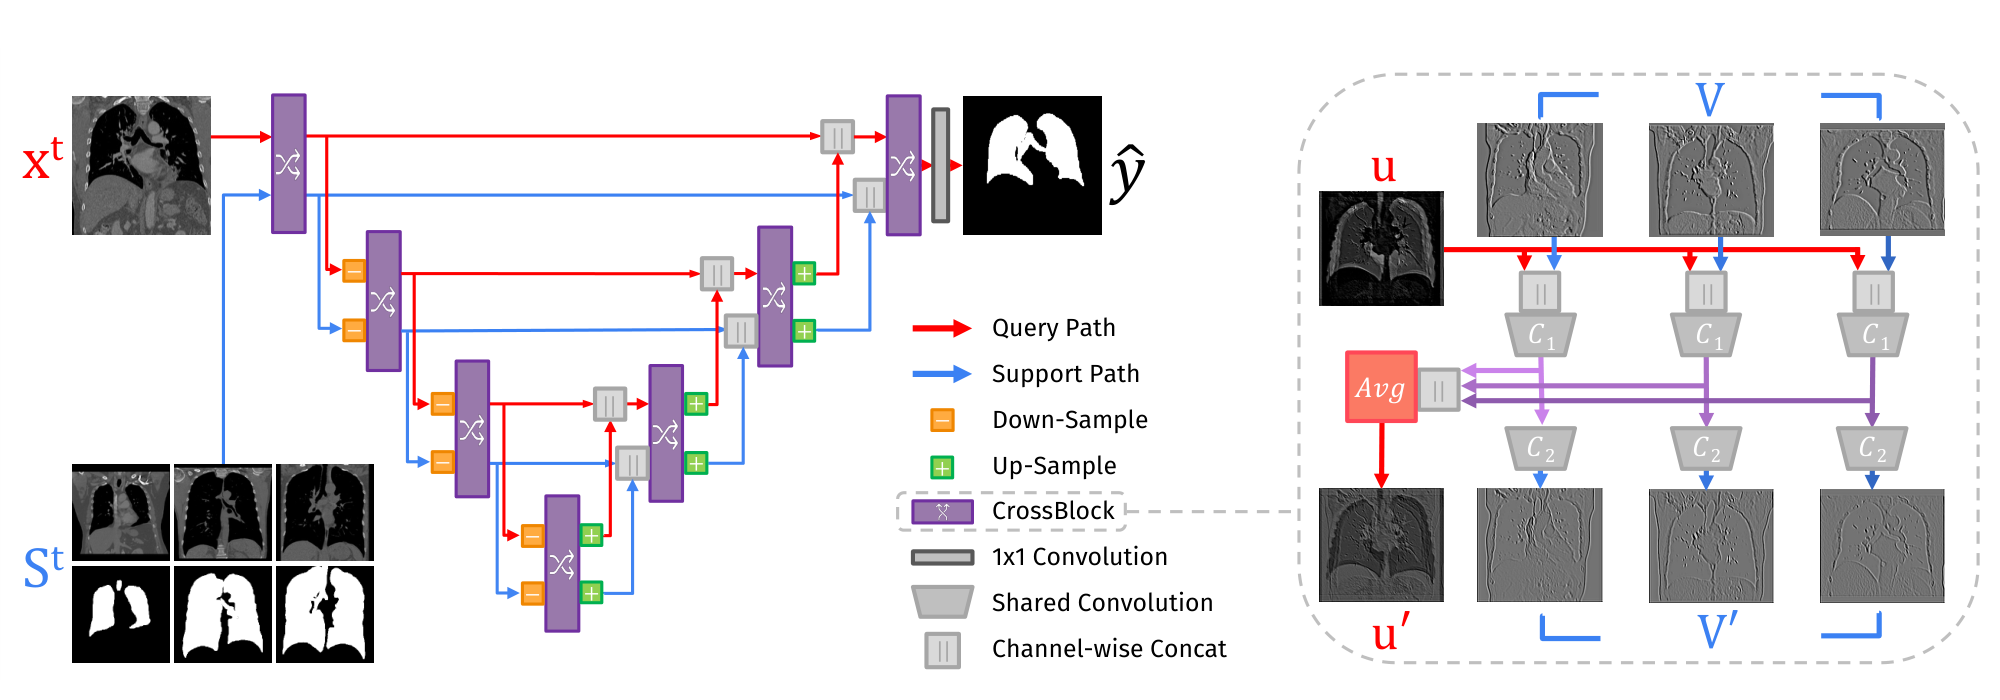
\includegraphics[width=1.0\linewidth, height=1.0\textheight, keepaspectratio]{images/Uniseg}

\end{frame}
% --- M3: ICS Architecture ---
\subsection{ICS Architecture}
\begin{frame}
    \frametitle{ICS Architecture}

    \begin{tikzpicture}[remember picture, overlay]
        \node[anchor=center, yshift=-0.4cm] at (current page.center) {%
            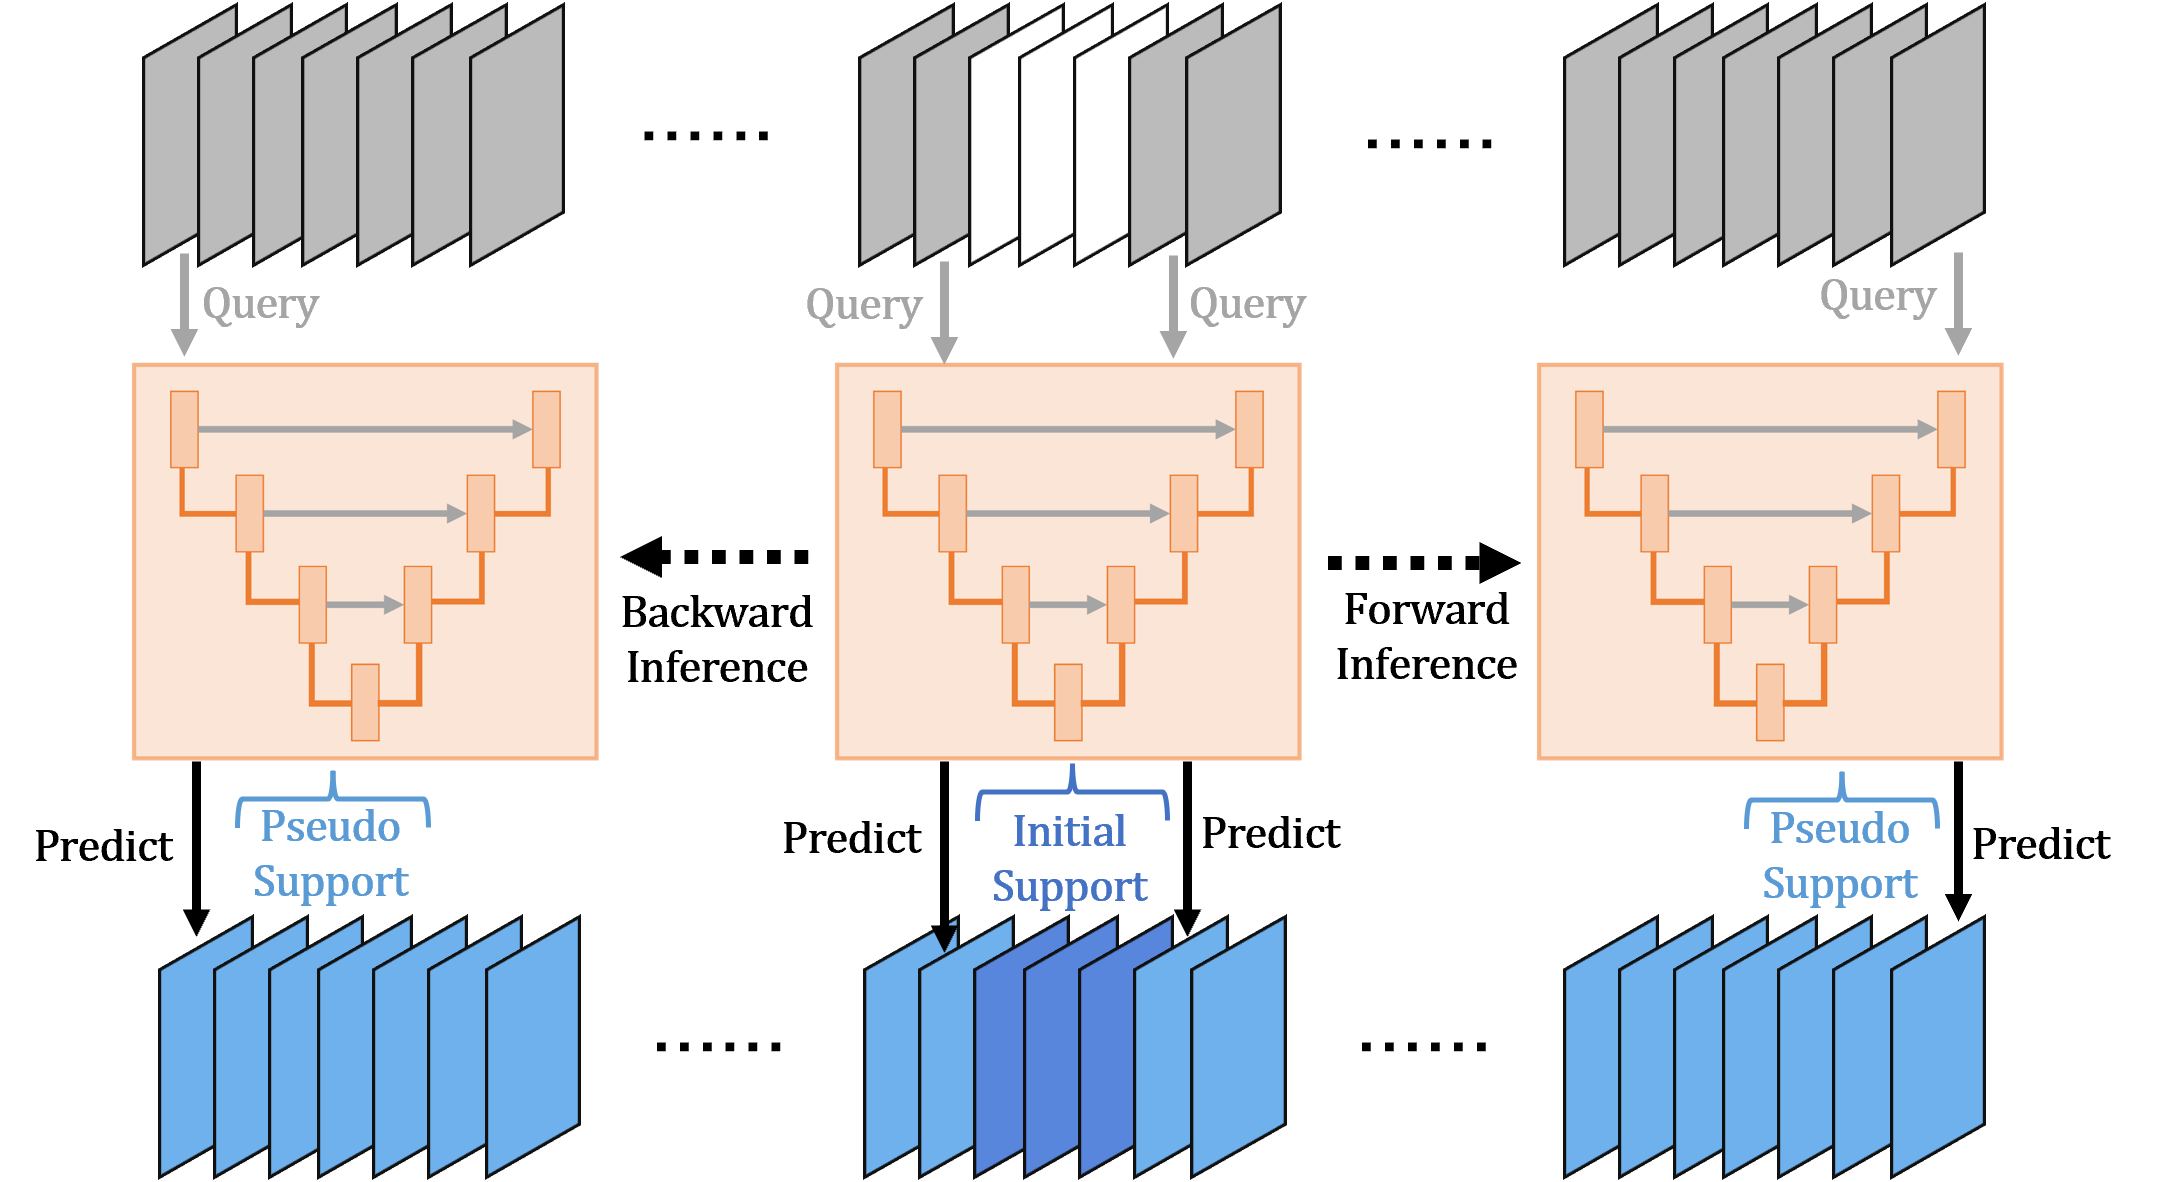
\includegraphics[width=0.80\textwidth]{fig2.png}%
        };
    \end{tikzpicture}

\end{frame}

% --- M4: Problem Formulation ---
\subsection{Problem Formulation}
\begin{frame}
    \frametitle{Problem Formulation}
    \framesubtitle{Implementation of ICS }

    We consider a volumetric dataset where each $\text{slice}_k$
    ($1 \le k \le n$) is a 2D cross-sectional image from CT or MRI:
    \[
        V = \{\text{slice}_1,\, \text{slice}_2,\, \ldots,\, \text{slice}_n\}
    \]

    Only $m$ slices have ground-truth labels forming the
    \textcolor{orange1}{\textbf{support set}} $S$:
    \[
        S = \bigl\{(\text{slice}_{\ell_1}, \text{label}_{\ell_1}),\;
                   (\text{slice}_{\ell_2}, \text{label}_{\ell_2}),\;
                   \ldots,\;
                   (\text{slice}_{\ell_m}, \text{label}_{\ell_m})\bigr\}
    \]
    where $\ell_1, \ell_2, \ldots, \ell_m$ are the labeled slice indices satisfying
    $1 \le \ell_1 < \ell_2 < \cdots < \ell_m \le n$.

    \vspace{0.3em}

    \textbf{Objective:} generate masks for all remaining $(n - m)$ unlabeled slices
    $k \in \{1,\ldots,n\} \setminus \{\ell_1,\ldots,\ell_m\}$:
    \[
        \hat{M}_k = f\!\left(\text{slice}_k,\; S\right)
    \]

    Here $f$ is the pretrained \textcolor{orange1}{\textbf{UniverSeg}} model.\textsuperscript{[1,7]}
    $\hat{M}_k$ has the same dimensions as $\text{slice}_k$ and assigns each pixel
    to its most likely anatomical class or background.

\end{frame}

% --- M5: Forward and Backward Inference ---
\subsection{Forward and Backward Inference}
\begin{frame}
    \frametitle{Forward \& Backward Inference}
    \framesubtitle{How ICS Propagates Through the Volume}

    \begin{block}{Forward Pass}
        Starting from the highest-indexed initial support slice
        UniverSeg infers masks in \textcolor{orange1}{\textbf{increasing}}
        slice order toward slice $n$. After each inference the predicted
        mask is added to \textbf{ForwardSupportSet}. Once $|S| > m$
        the oldest entry is discarded.
    \end{block}

    \vspace{0.5em}

    \begin{block}{Backward Pass}
        Starting from the lowest-indexed initial slice inference proceeds
        in \textcolor{orange1}{\textbf{decreasing}} order toward slice $1$
        using \textbf{BackwardSupportSet} with the same rolling window logic.
    \end{block}

    \vspace{0.5em}

    \begin{exampleblock}{Augmentation}
        During each inference support images are rotated by
        \textbf{90°, 180° and 270°} to improve robustness
        against orientation variation.
    \end{exampleblock}

\end{frame}


% ============================================================
% SECTION BREAK
% ============================================================
\section{Dataset \& Experiments}
\begin{breakframe}
    Experiments
\end{breakframe}

% ============================================================
% SECTION 4 — EXPERIMENTS
% ============================================================

% --- Slide 13 ---
\subsection{Dataset}
\begin{frame}
    \frametitle{The HVSMR Dataset}
    \framesubtitle{How our heart looks visually }

    \begin{columns}[c]
        \column{0.45\textwidth}
            The \textcolor{orange1}{\textbf{HVSMR}} dataset contains
            \textbf{60 cardiovascular MRI scans} from Boston Children's
            Hospital covering patients with congenital heart conditions.


            \vspace{0.6em}

            Ground-truth masks were generated by combining manual
            annotations with automated \textbf{3D-UNet} output followed by
            expert revision.

        \column{0.55\textwidth}
            \centering
            \animategraphics[loop, autoplay, width=\linewidth]{15}{/Users/hemanthmg/Documents/SlicerCapture/image_}{00000}{00119}
    \end{columns}

\end{frame}

% --- Slide 13b ---
\subsection{8 Cardiac Regions}
\begin{frame}
    \frametitle{8 Cardiac Regions}
    \framesubtitle{3D Visualization of Heart regions}

    \makebox[\textwidth][l]{\hspace*{-0.5cm}%
    \begin{columns}[c]

        % LEFT COLUMN — Pair 1 and Pair 3
        \column{0.5\textwidth}

            % Pair 1
            \begin{columns}[c]
                \column{0.65\textwidth}
                    \animategraphics[loop, autoplay, width=\linewidth]{15}{/Users/hemanthmg/Documents/SlicerCapture/pair1/image_}{00000}{00119}
                \column{0.35\textwidth}
                    {\small\textcolor{red}{\rule{0.7em}{0.7em}}~Left Ventricle}\\[0.4em]
                    {\small\textcolor{orange1}{\rule{0.7em}{0.7em}}~Aorta}
            \end{columns}

            \vspace{0.4em}

            % Pair 3
            \begin{columns}[c]
                \column{0.65\textwidth}
                    \animategraphics[loop, autoplay, width=\linewidth]{15}{/Users/hemanthmg/Documents/SlicerCapture/pair3/image_}{00000}{00119}
                \column{0.35\textwidth}
                    {\small\textcolor[rgb]{0.95,0.45,0.65}{\rule{0.7em}{0.7em}}~Left Atrium}\\[0.4em]
                    {\small\textcolor{cyan1}{\rule{0.7em}{0.7em}}~Right Atrium}
            \end{columns}

        % RIGHT COLUMN — Pair 2 and Pair 4
        \column{0.5\textwidth}

            % Pair 2
            \begin{columns}[c]
                \column{0.65\textwidth}
                    \animategraphics[loop, autoplay, width=\linewidth]{15}{/Users/hemanthmg/Documents/SlicerCapture/pair2/image_}{00000}{00119}
                \column{0.35\textwidth}
                    {\small\textcolor{blau1}{\rule{0.7em}{0.7em}}~Right Ventricle}\\[0.4em]
                    {\small\textcolor{gruen1}{\rule{0.7em}{0.7em}}~Pulmonary Artery}
            \end{columns}

            \vspace{0.4em}

            % Pair 4
            \begin{columns}[c]
                \column{0.65\textwidth}
                    \animategraphics[loop, autoplay, width=\linewidth]{15}{/Users/hemanthmg/Documents/SlicerCapture/pair4/image_}{00000}{00119}
                \column{0.35\textwidth}
                    {\small\textcolor{lila1}{\rule{0.7em}{0.7em}}~Superior Vena Cava}\\[0.4em]
                    {\small\textcolor[rgb]{0.9,0.8,0.05}{\rule{0.7em}{0.7em}}~Inferior Vena Cava}
            \end{columns}

    \end{columns}}

\end{frame}

% --- Slide 14 ---

% --- Slide 15 ---
\subsection{Experimental Settings}
\begin{frame}
    \frametitle{Experimental Settings}
    \framesubtitle{Three Evaluation Protocols}
    \vspace{0.6em}

    \textcolor{orange1}{\textbf{Quantitative \& Qualitative Comparison}}\\
    Compares ICS against the baseline UniverSeg approach using identical
    initial support slices and augmentation settings to assess accuracy
    and boundary segmentation quality.

    \vspace{0.5em}

    \textcolor{orange1}{\textbf{Effect of Support Slice Count}}\\
    Evaluates how varying the number of initial support slices ($m = 1$ to $5$)
    affects performance and identifies potential diminishing returns.

    \vspace{0.5em}

    \textcolor{orange1}{\textbf{Effect of Initial Slice Position}}\\
    Investigates how the spatial positioning of initial labeled slices influences
    segmentation. \textbf{Patient\_32} is used as a representative case for
    detailed visualization.

\end{frame}

% --- Slide 16 ---
\subsection{Dice Similarity Coefficient}
\begin{frame}
    \frametitle{Dice Similarity Coefficient}
    \framesubtitle{Primary Evaluation Metric}

    The \textcolor{orange1}{\textbf{Dice Similarity Coefficient (DSC)}} serves as
    the primary metric for quantitative evaluation of segmentation accuracy.

    \vspace{0.7em}

    DSC is calculated on a \textbf{pixel by pixel} basis by comparing predicted
    masks against ground truth labels.

    \vspace{0.7em}

    \[\displaystyle
        \text{DSC} = \frac{2 \cdot \text{TP}}{2 \cdot \text{TP} + \text{FP} + \text{FN}}
    \]

    \vspace{0.4em}

    where \textbf{TP} (True Positives), \textbf{FP} (False Positives) and
    \textbf{FN} (False Negatives).

\end{frame}

% ============================================================
% SECTION BREAK
% ============================================================
\section{Results}
\begin{breakframe}
    Results
\end{breakframe}

% ============================================================
% SECTION 5 — RESULTS
% ============================================================

% --- Slide 17 ---
\subsection{Quantitative Results}
\begin{frame}
    \frametitle{Quantitative Results}
    \framesubtitle{DSC Table 1 and Box Plots\textsuperscript{[1,3]}}

    \begin{columns}[c]

        \column{0.40\textwidth}
            \centering
            {\scriptsize
            \setlength{\arrayrulewidth}{0.8pt}
            \begin{tabular}{>{\bfseries}l ccc cc}
                \toprule
                \multicolumn{1}{l}{Region} & \multicolumn{2}{c}{Baseline} & \multicolumn{2}{c}{ICS} & p-value \\
                \cmidrule(lr){2-3}\cmidrule(lr){4-5}
                & Mean & Std & Mean & Std & \\
                \midrule
                \textcolor{red}{\rule{0.5em}{0.5em}}~LV
                    & 0.5489 & 0.0893 & 0.5475 & 0.0770 & 0.8903 \\[2pt]
                \textcolor{blau1}{\rule{0.5em}{0.5em}}~RV
                    & 0.4663 & 0.1047 & 0.4741 & 0.0933 & 0.3820 \\[2pt]
                \textcolor[rgb]{0.95,0.45,0.65}{\rule{0.5em}{0.5em}}~LA
                    & 0.3879 & 0.1210 & \textbf{0.4272} & 0.0925 & 0.0007 \\[2pt]
                \textcolor{cyan1}{\rule{0.5em}{0.5em}}~RA
                    & 0.5500 & 0.1191 & \textbf{0.5734} & 0.0791 & 0.0214 \\[2pt]
                \textcolor{orange1}{\rule{0.5em}{0.5em}}~AO
                    & 0.4945 & 0.1269 & \textbf{0.5210} & 0.0679 & 0.0206 \\[2pt]
                \textcolor{gruen1}{\rule{0.5em}{0.5em}}~PA
                    & 0.3807 & 0.1336 & \textbf{0.4745} & 0.0974 & $<$0.0001 \\[2pt]
                \textcolor{lila1}{\rule{0.5em}{0.5em}}~SVC
                    & 0.4079 & 0.1805 & \textbf{0.4938} & 0.1226 & $<$0.0001 \\[2pt]
                \textcolor[rgb]{0.9,0.8,0.05}{\rule{0.5em}{0.5em}}~IVC
                    & 0.4607 & 0.1258 & 0.4629 & 0.0871 & 0.8561 \\
                \bottomrule
            \end{tabular}
            }

        \column{0.58\textwidth}
            \centering
            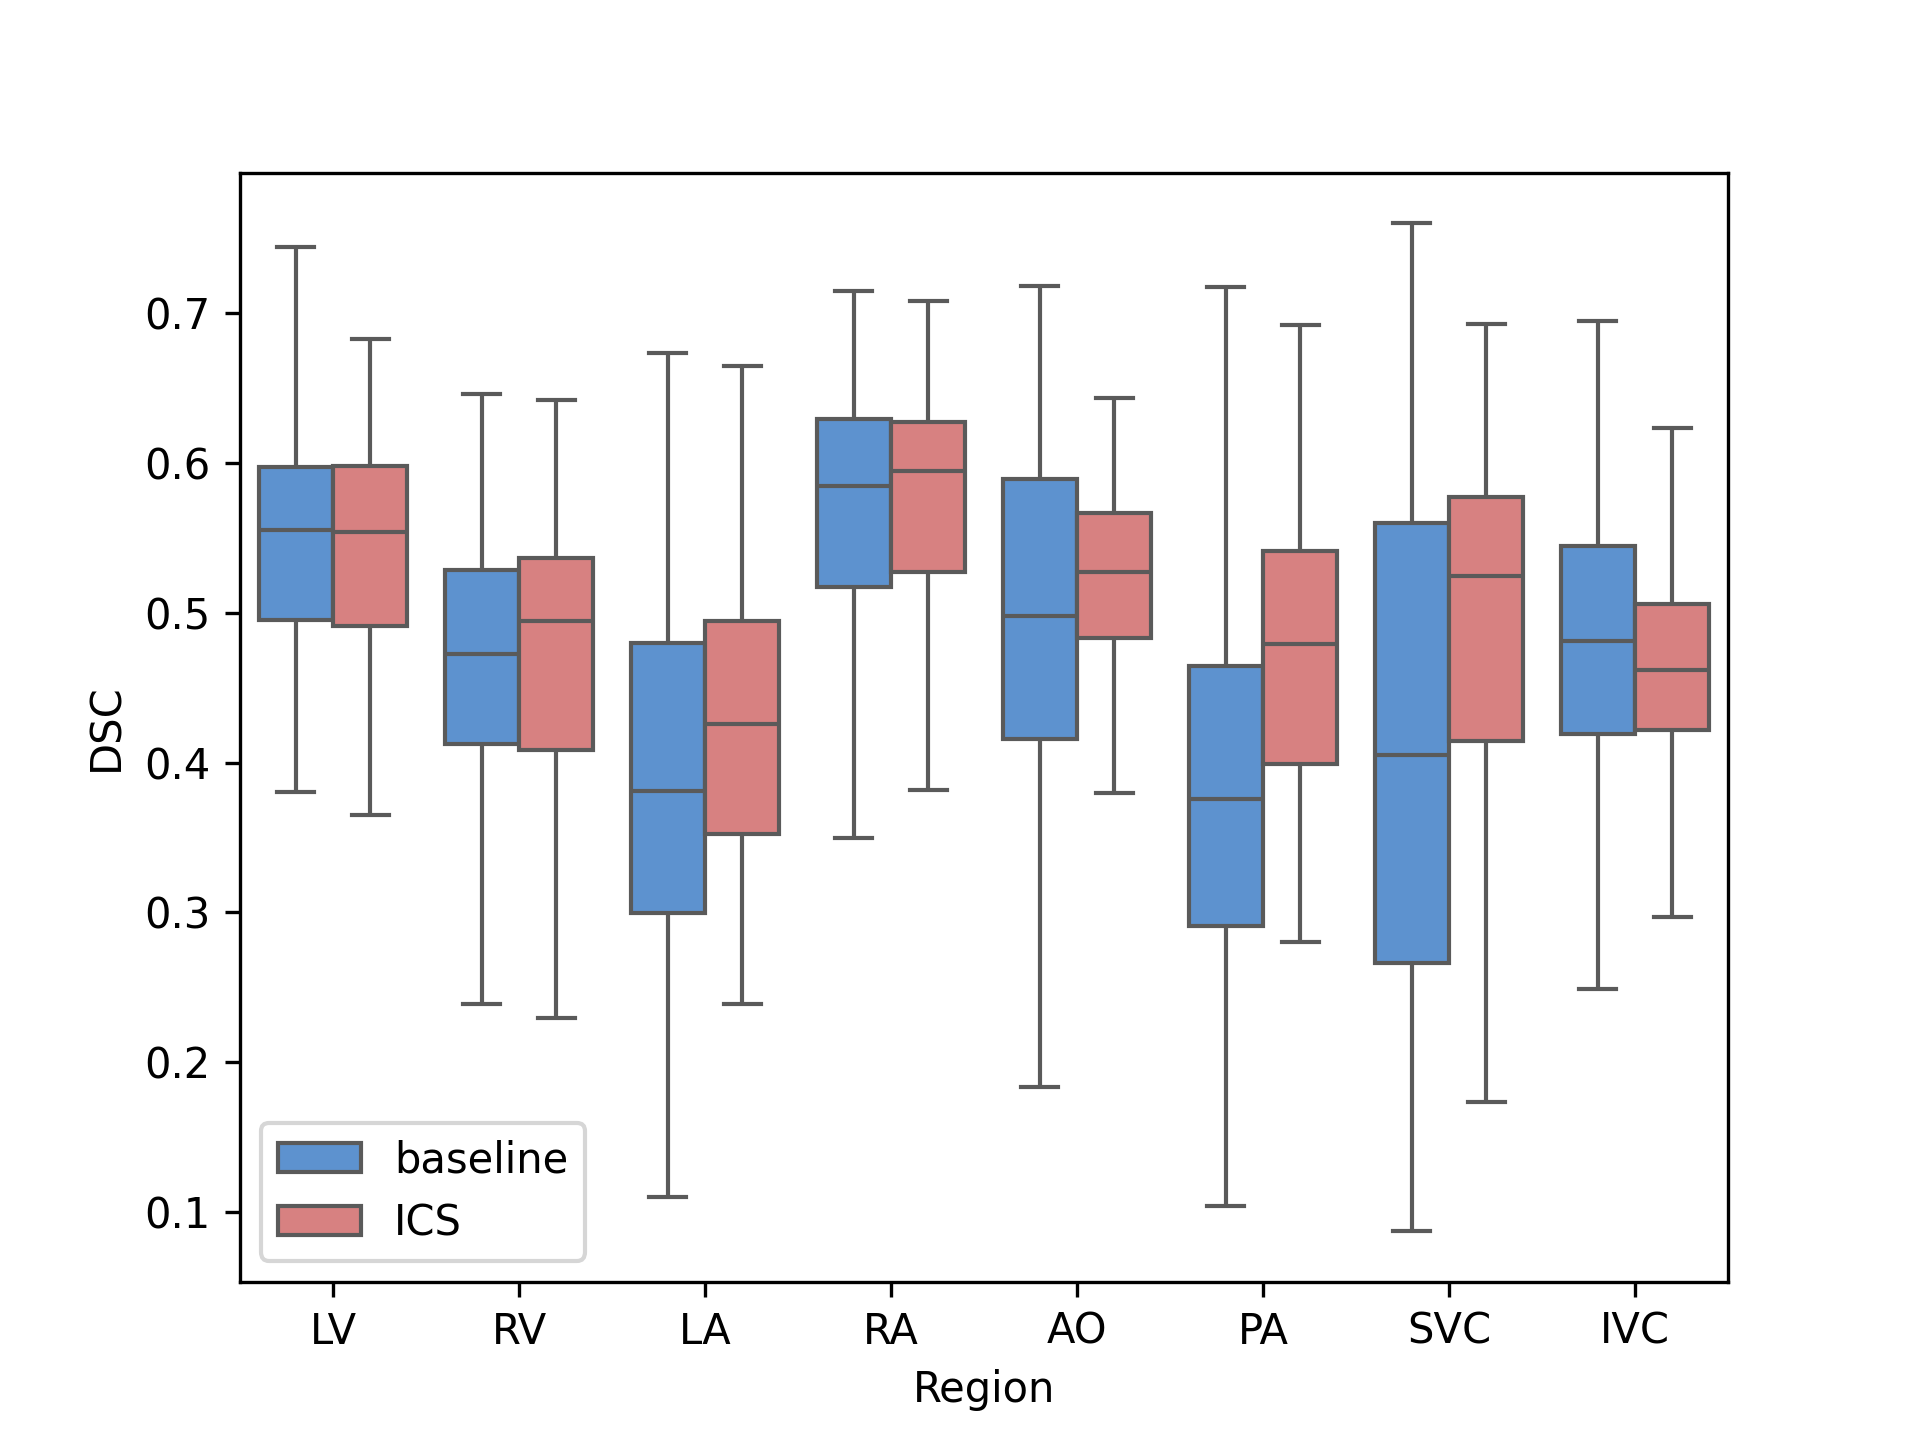
\includegraphics[width=\linewidth]{fig3.png}

    \end{columns}

\end{frame}

% --- Slide 18 ---
\subsection{Qualitative Results}
\begin{frame}
    \frametitle{Qualitative Results}
    \framesubtitle{Segmentated LV and PA Regions respectivley }

    \begin{columns}[c]
        \column{0.45\textwidth}
            \centering
            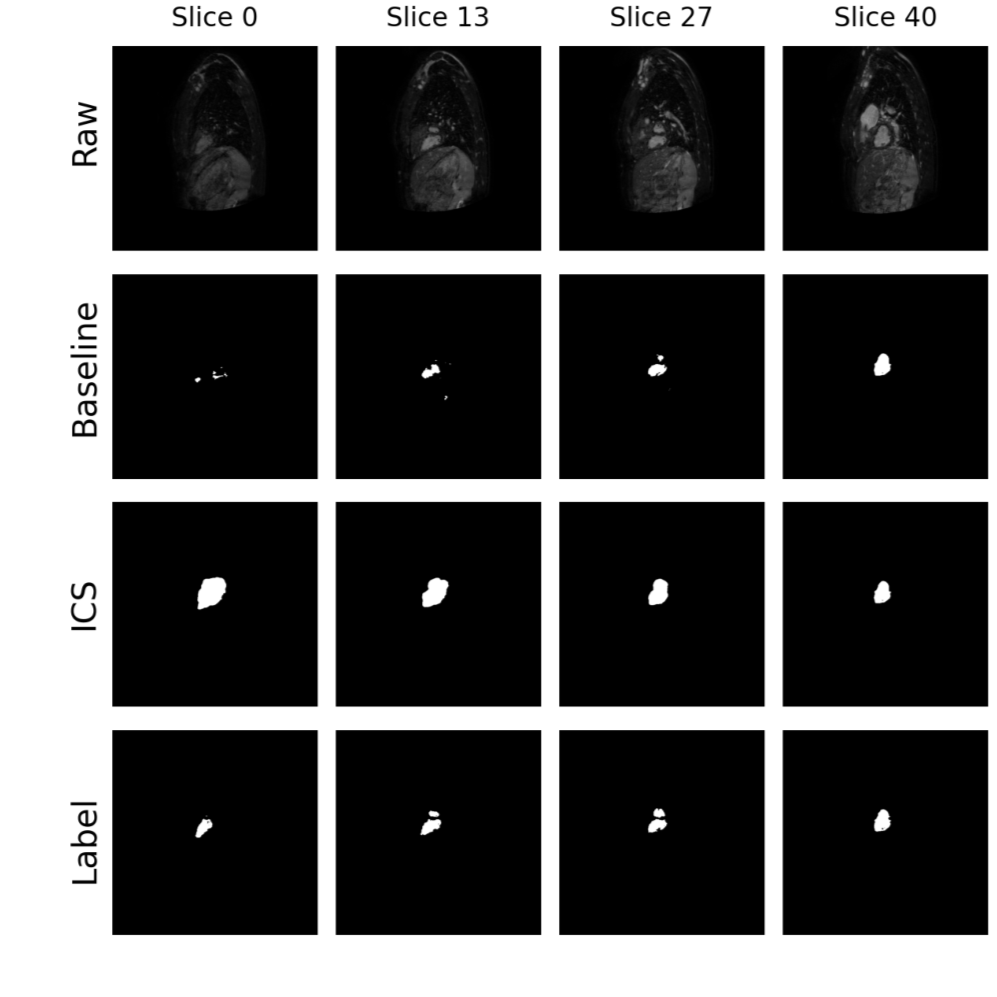
\includegraphics[width=\linewidth]{LV.png}

        \column{0.45\textwidth}
            \centering
            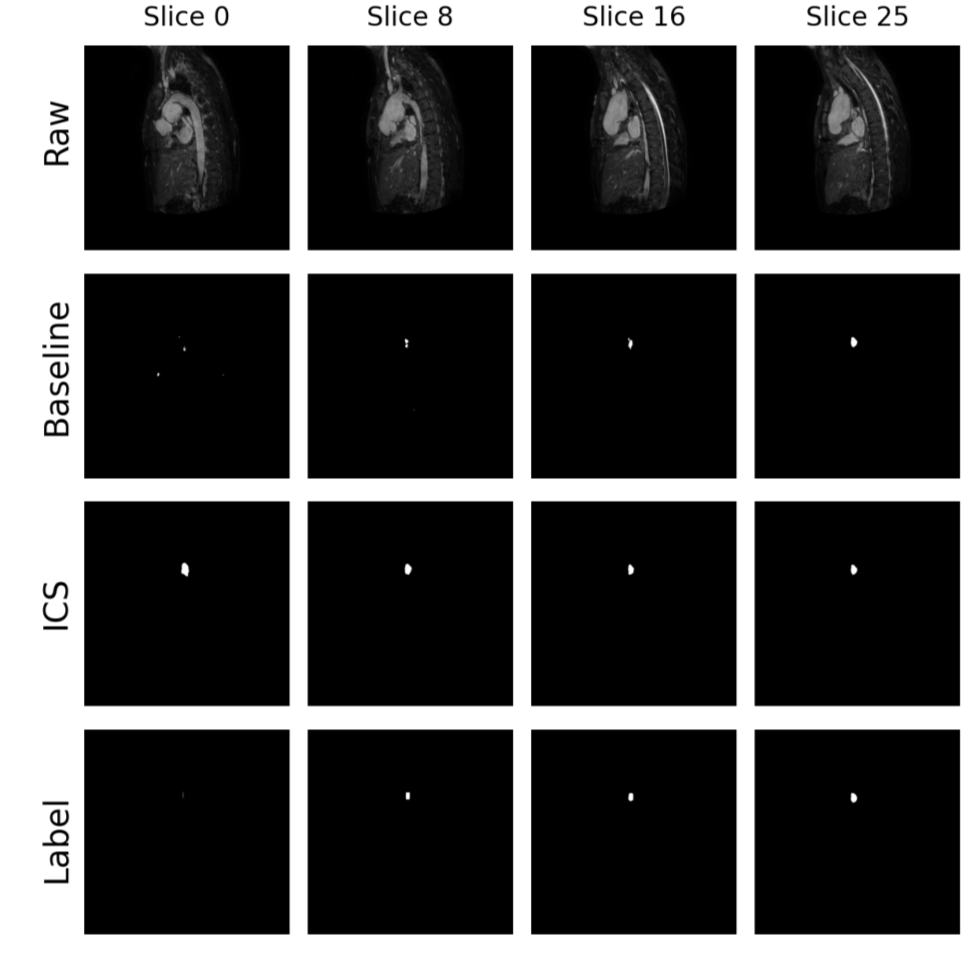
\includegraphics[width=\linewidth]{PA.png}
    \end{columns}

\end{frame}

% --- Slide 19 ---
\subsection{Slice-by-Slice Consistency}
\begin{frame}
    \frametitle{Slice-by-Slice Consistency}
    \framesubtitle{Fig.~6 Line Plots}
    \centering
    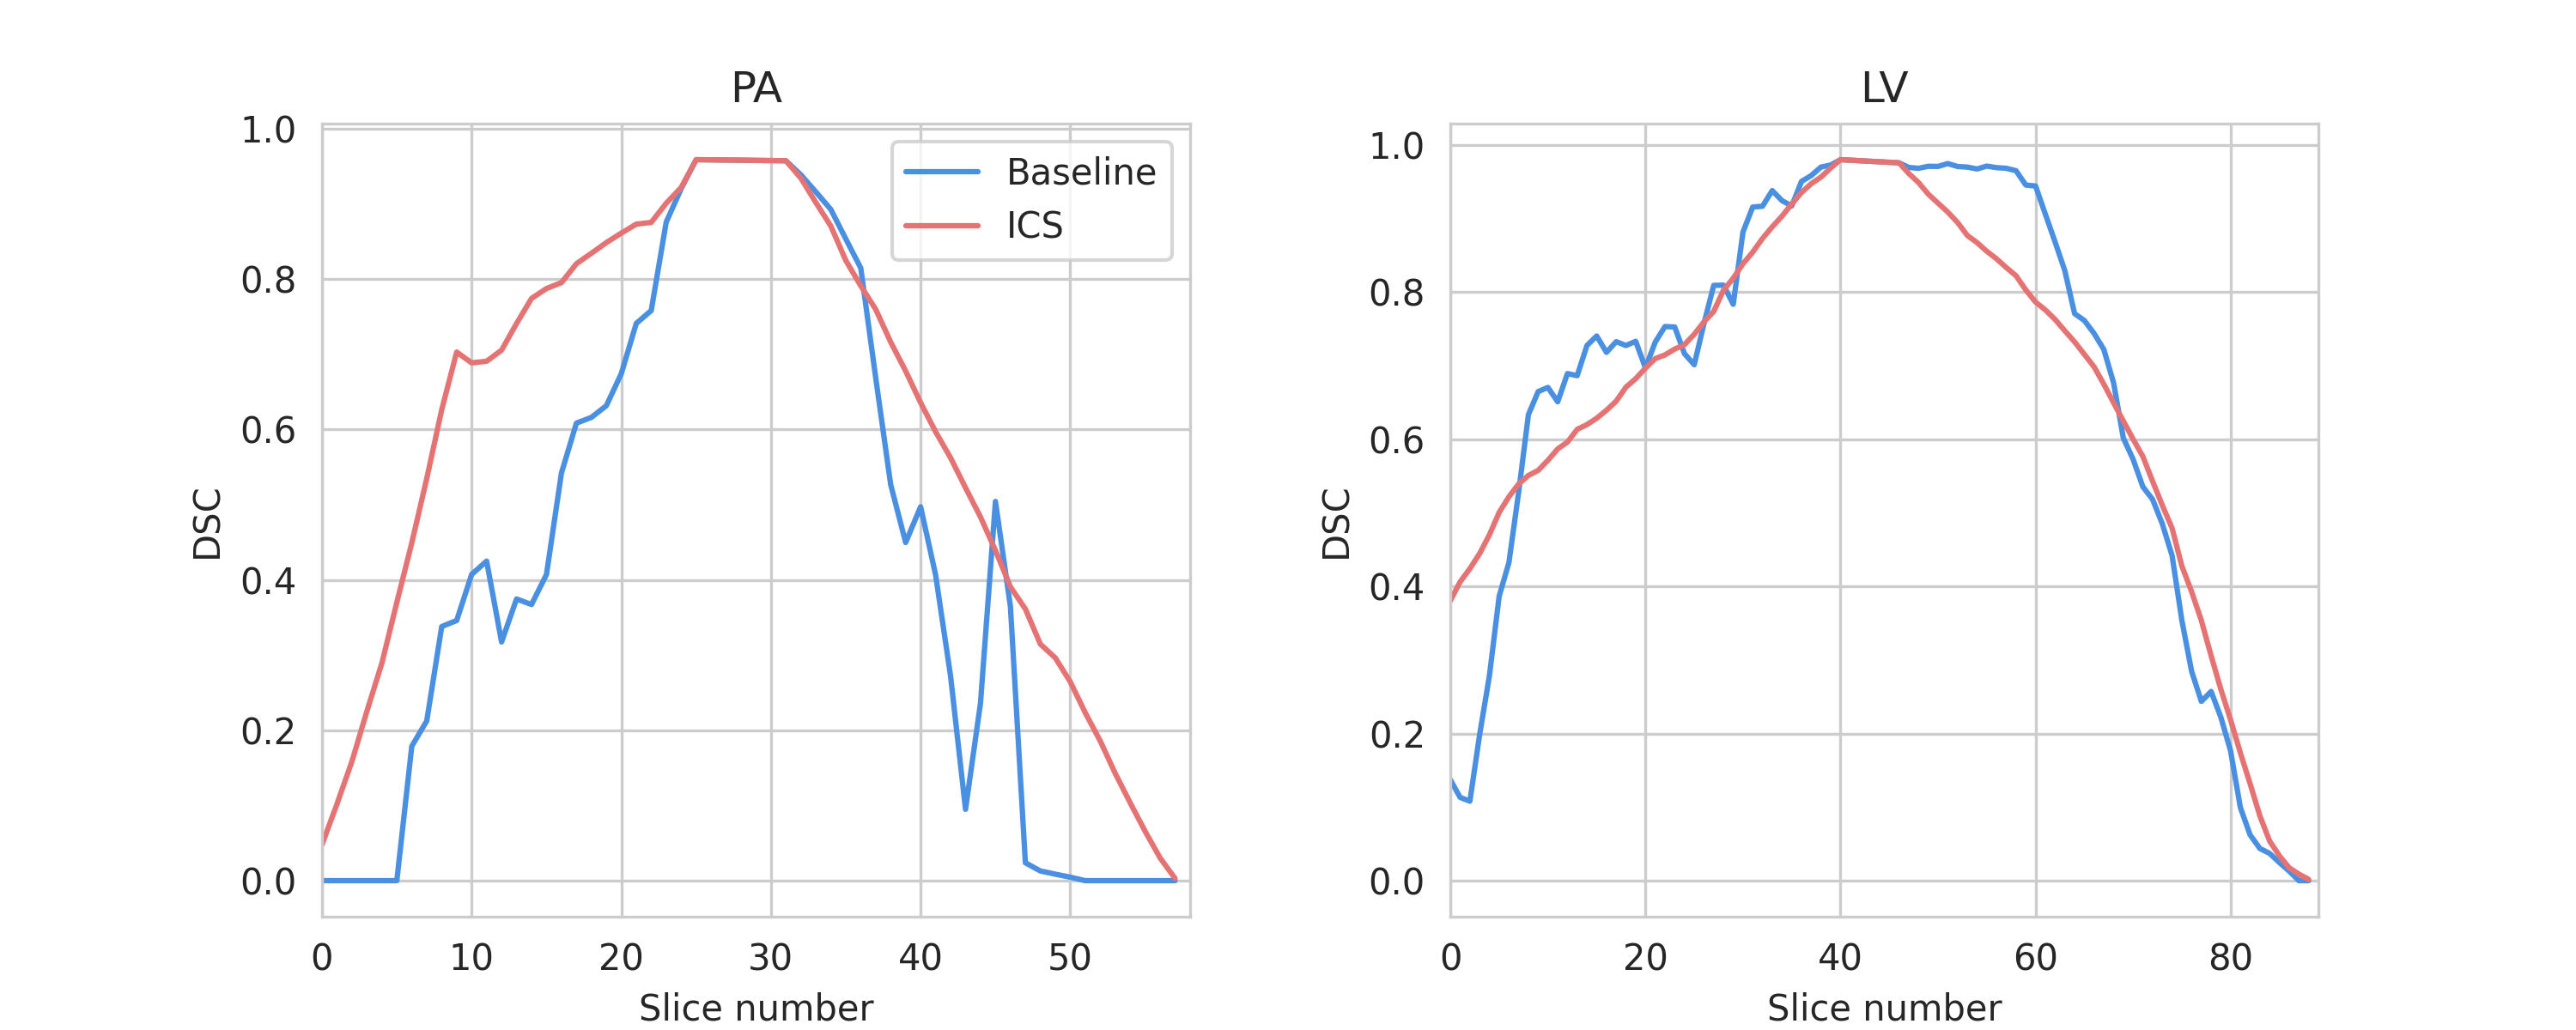
\includegraphics[width=1.1\textwidth]{fig6.png}
\end{frame}

% --- Slide 20 ---
\subsection{Effect of Initial Slice Position}
\begin{frame}
    \frametitle{Effect of Initial Slice Position}
    \framesubtitle{Fig.~8 — Placement Sensitivity}
    \centering
    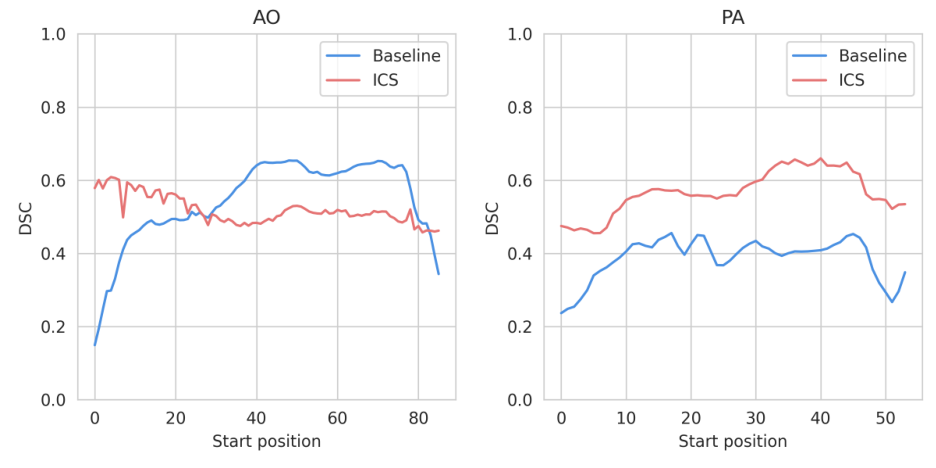
\includegraphics[width=0.88\textwidth]{fig8.png}
\end{frame}

% ============================================================
% SECTION BREAK
% ============================================================
\section{Discussion \& Conclusion}
\begin{breakframe}
    Discussion \& Conclusion
\end{breakframe}

% ============================================================
% SECTION 6 — DISCUSSION AND CONCLUSION
% ============================================================

% --- Slide 21 ---
\subsection{Discussion}
\begin{frame}
    \frametitle{Discussion}
    \framesubtitle{Strengths and Limitations}

    ICS \textcolor{orange1}{\textbf{significantly outperformed}} the baseline in five
    anatomical regions by maintaining inter-slice consistency and accurately
    capturing complex structures.

    \vspace{0.5em}

    In regions like the \textbf{LV} and \textbf{IVC} ICS exhibited a tendency to
    \textcolor{orange1}{\textbf{over-segment}} and produce false positives suggesting
    a need for future confidence metrics during support set updates.

    \vspace{0.5em}

    Increasing the number of initial support slices improved accuracy and stability
    but introduced \textcolor{orange1}{\textbf{computational trade-offs}} in inference
    time and GPU memory usage.

    \vspace{0.5em}

    The \textcolor{orange1}{\textbf{spatial location}} of initial support slices heavily
    impacted accuracy with performance generally degrading as the distance from the
    initial position increased.

\end{frame}

% --- Slide 22 ---
\subsection{Future Work}
\begin{frame}
    \frametitle{Future Work}
    \framesubtitle{Slice Selection, Efficiency, Cross-modality}

    Future research must address the \textcolor{orange1}{\textbf{cold-start problem}}
    by using approaches like clustering to automatically identify the best initial
    slices to annotate.

    \vspace{0.6em}

    The current method assumes all slices contain the target region requiring a
    mechanism to \textcolor{orange1}{\textbf{halt label propagation}} when processing
    slices that lack the region of interest.

    \vspace{0.6em}

    Because UniverSeg was pre-trained on most public datasets validation was
    restricted to a \textcolor{orange1}{\textbf{single dataset}} requiring future
    testing on private datasets and diverse modalities like ultrasound and CT.

\end{frame}

% --- Slide 23 ---
\subsection{Conclusion}
\begin{frame}
    \frametitle{Conclusion}
    \framesubtitle{Key Takeaways}

    \begin{columns}[t]

        \column{0.48\textwidth}
            \begin{itemize}
                \item ICS reduces annotation burdens by propagating segmentation context
                      \textcolor{orange1}{\textbf{bidirectionally}} across slices.
                \item Experiments show \textcolor{orange1}{\textbf{significant improvements}}
                      in slice-to-slice consistency and complex structure capture.
                \item Success depends on enough initial support slices and
                      \textcolor{orange1}{\textbf{positioning them effectively}}.
            \end{itemize}

        \column{0.48\textwidth}
            \begin{itemize}
                \item Key limits include \textcolor{orange1}{\textbf{over-segmentation}}
                      computational memory costs and finding the right initial slices.
                \item Future research focuses on optimizing support set updates and
                      \textcolor{orange1}{\textbf{automating slice selection}}.
                \item ICS is a strong framework for \textcolor{orange1}{\textbf{low-annotation
                      clinical segmentation}} with broader modality testing planned.
            \end{itemize}

    \end{columns}

\end{frame}

% Questions Slide
\begin{frame}
    \frametitle{}
    \framesubtitle{}

    \vspace*{\fill}
    \centering

    {\LARGE\bfseries\textcolor{orange1}{Thank you for your attention!}}

    \vspace{0.6em}

    {\large\textcolor{grau1}{I am open to your questions!}}

    \vspace{0.5em}

    
\includegraphics[height=5.2em]{text.png}

    \vspace*{\fill}

\end{frame}

% Thank You
\begin{thankyouframe}
\end{thankyouframe}

% ============================================================
% BACKUP SLIDES
% ============================================================

\begin{frame}
    \frametitle{Effect of Support Slice Count}
    \framesubtitle{DSC vs. Number of Initial Support Slices}
    \centering
    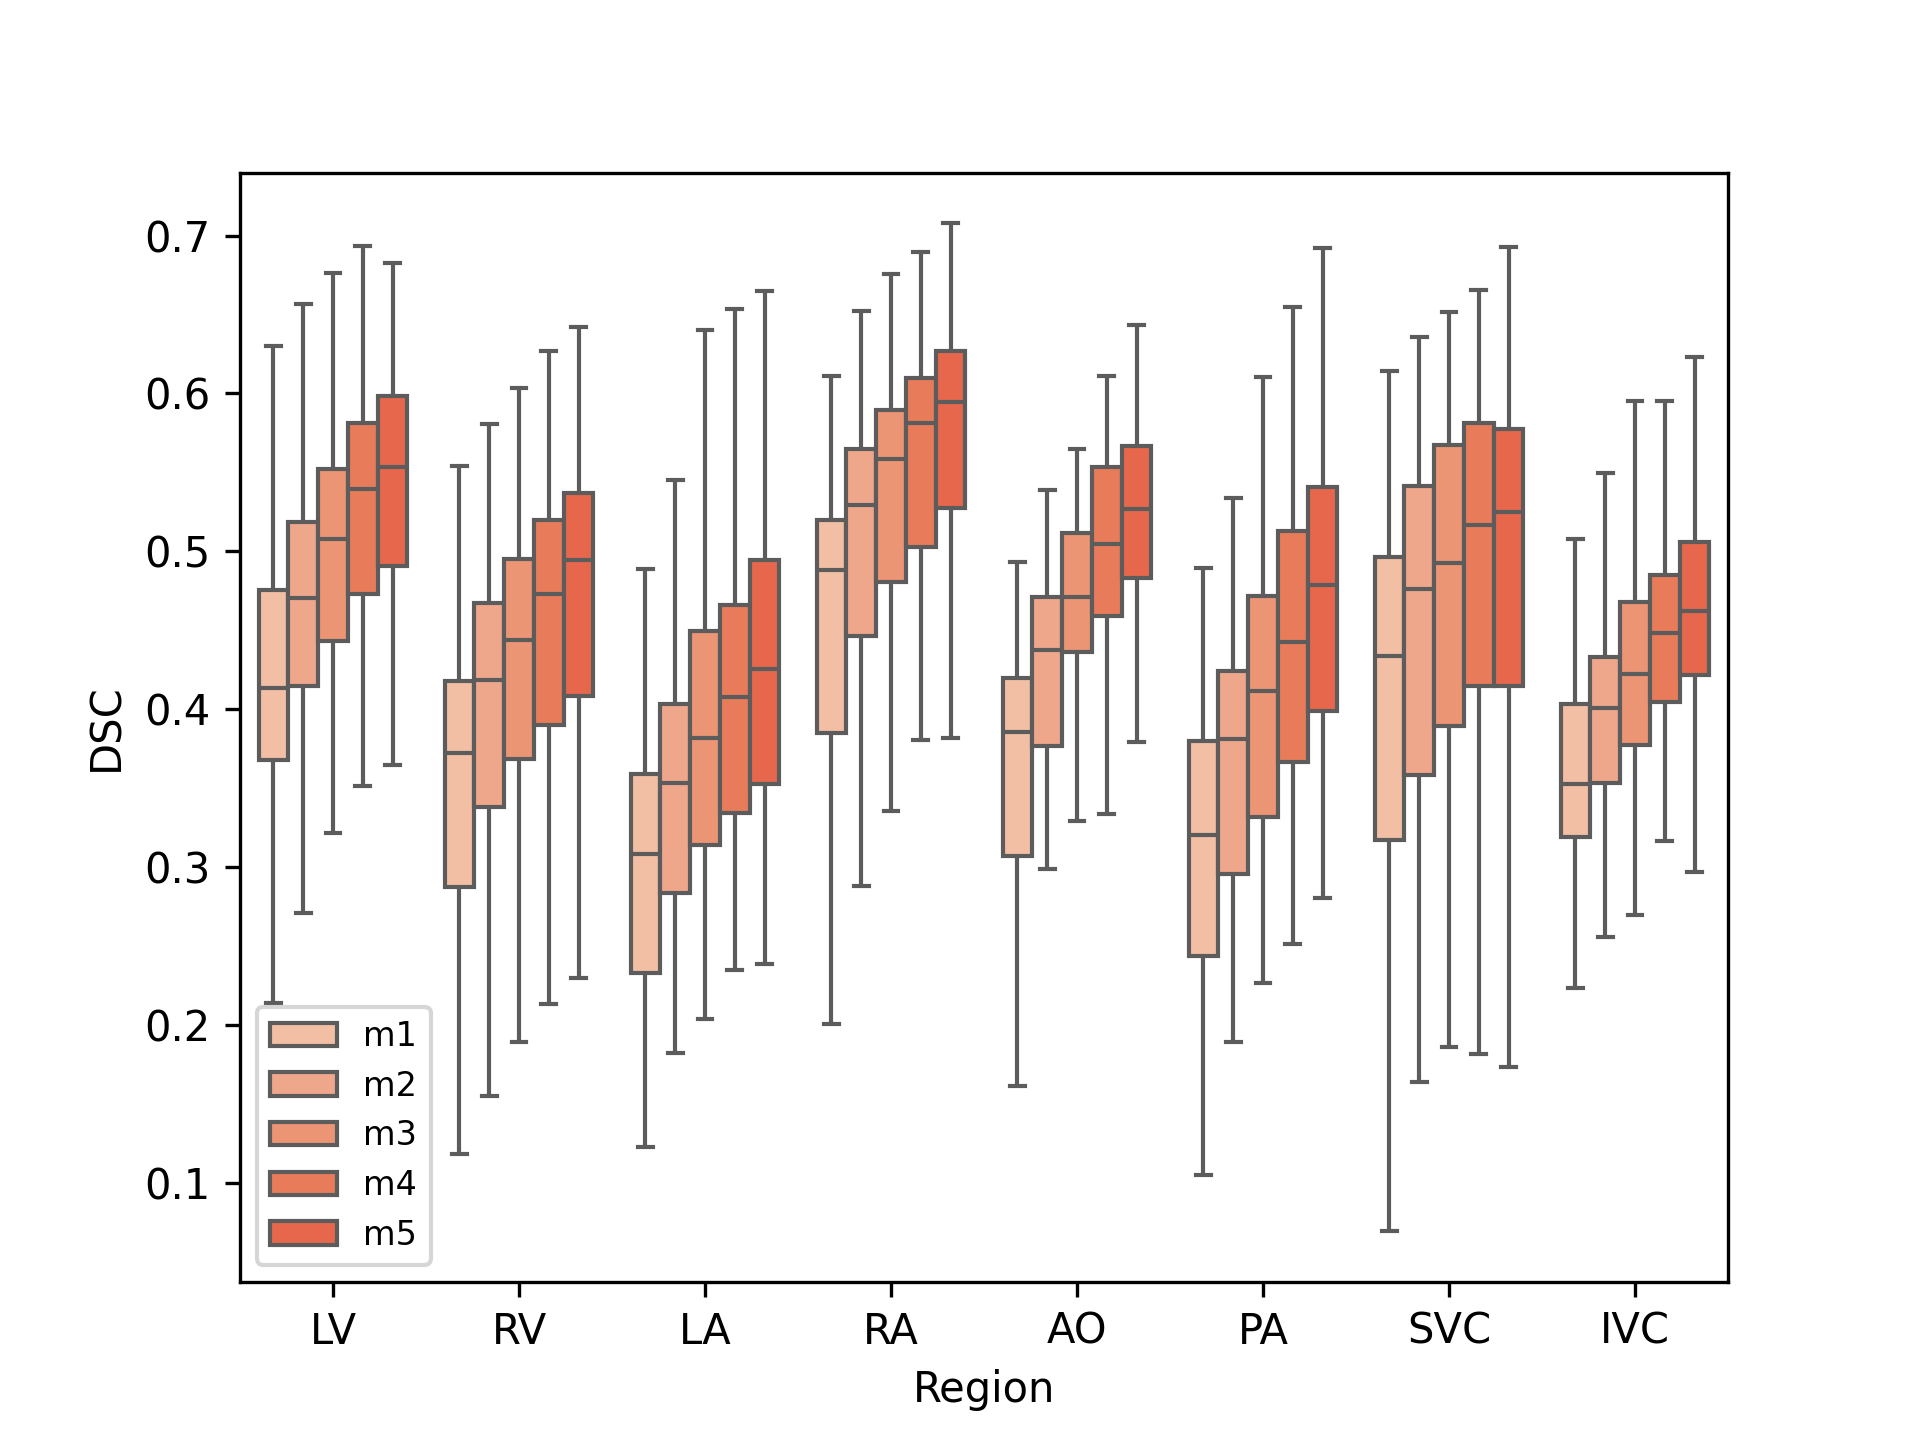
\includegraphics[width=\textwidth, height=0.82\textheight, keepaspectratio]{fig7.png}
\end{frame}

% Backup Slide 2 — Algorithm Part 1
\subsection{ICS Algorithm}
\begin{frame}
    \frametitle{ICS Algorithm }
    \framesubtitle{Initialization \& Forward Pass}

    {\small
    \textbf{Require:} Volume $V$, InitialSupportSet, UniverSeg, max size $m$, Augment()

    \vspace{0.5em}
    \textbf{Initialize:} ForwardSupportSet $\leftarrow$ InitialSupportSet\\
    \phantom{\textbf{Initialize:}} BackwardSupportSet $\leftarrow$ InitialSupportSet

    \vspace{0.6em}
    \textcolor{cyan1}{\textbf{Forward pass}} ($i = \max(c_k)$ to $n$):
    \begin{enumerate}\itemsep6pt
        \item Query $\leftarrow$ slice$_i$
        \item $\hat{y} \leftarrow$ UniverSeg(Query, Augment(ForwardSupportSet))
        \item Append $(\text{slice}_i, \hat{y})$ to ForwardSupportSet
        \item If $|$ForwardSupportSet$| > m$: remove oldest entry
    \end{enumerate}
    }

\end{frame}

% Backup Slide 3 — Algorithm Part 2
\begin{frame}
    \frametitle{ICS Algorithm }
    \framesubtitle{Backward Pass \& Key Properties}

    {\small
    \textcolor{lila1}{\textbf{Backward pass}} ($i = \min(c_k)$ down to $1$):
    \begin{enumerate}\itemsep6pt
        \item Query $\leftarrow$ slice$_i$
        \item $\hat{y} \leftarrow$ UniverSeg(Query, Augment(BackwardSupportSet))
        \item Append $(\text{slice}_i, \hat{y})$ to BackwardSupportSet
        \item If $|$BackwardSupportSet$| > m$: remove oldest entry
    \end{enumerate}

    \vspace{0.5em}
    \textbf{Return:} ForwardPredictedLabels, BackwardPredictedLabels

    \vspace{0.6em}
    \textcolor{orange1}{\textbf{Rolling window}} ($m = 5$): oldest entries discarded to keep context spatially local.
    Augmentation: rotations 90°/180°/270° at each step.
    UniverSeg weights remain \textbf{frozen} throughout.
    }

\end{frame}

% Backup Slide 4 — Generalization Gap Diagram
\begin{frame}
    \frametitle{The Generalization Gap}
    \framesubtitle{Why Fixed Models Break in the Real World}

    \centering
    \begin{tikzpicture}[
        train/.style={draw=orange1, fill=orange4, rounded corners=4pt,
                      minimum width=2.8cm, minimum height=0.9cm,
                      font=\small\bfseries, align=center, text=grau1},
        model/.style={draw=grau1, fill=grau4, rounded corners=4pt,
                      minimum width=2.2cm, minimum height=0.9cm,
                      font=\small\bfseries, align=center, text=grau1},
        fail/.style={draw=lila1, fill=lila1med, rounded corners=4pt,
                     minimum width=2.8cm, minimum height=0.9cm,
                     font=\small\bfseries, align=center, text=lila1},
        arr/.style={-{Stealth[length=6pt]}, grau2, line width=1pt},
        farr/.style={-{Stealth[length=6pt]}, lila1, line width=1pt, dashed},
        lbl/.style={font=\scriptsize, text=grau2, align=center}
    ]
        % ---- ROW 1: Domain Shift ----
        \node[train] (t1) {CT Scans\\{\tiny Hospital A}};
        \node[model, right=1.0cm of t1] (m1) {Trained\\Model};
        \node[fail, right=1.0cm of m1] (f1) {MRI Scans\\{\tiny Hospital B}};
        \draw[arr] (t1) -- (m1);
        \draw[farr] (m1) -- (f1);
        \node[text=lila1, font=\Large\bfseries, right=0.2cm of f1] {$\times$};
        \node[lbl, above=0.15cm of t1] {Train};
        \node[lbl, above=0.15cm of f1] {Deploy};
        \node[lbl, right=0.8cm of f1, text=lila1] {Domain\\shift};

        % ---- ROW 2: Modality Shift ----
        \node[train, below=1.0cm of t1] (t2) {Brain MRI\\{\tiny Tumour}};
        \node[model, right=1.0cm of t2] (m2) {Same\\Model};
        \node[fail, right=1.0cm of m2] (f2) {Cardiac MRI\\{\tiny New organ}};
        \draw[arr] (t2) -- (m2);
        \draw[farr] (m2) -- (f2);
        \node[text=lila1, font=\Large\bfseries, right=0.2cm of f2] {$\times$};
        \node[lbl, right=0.8cm of f2, text=lila1] {Modality\\shift};

        % ---- ROW 3: Site Shift ----
        \node[train, below=1.0cm of t2] (t3) {Scanner A\\{\tiny 1.5T MRI}};
        \node[model, right=1.0cm of t3] (m3) {Same\\Model};
        \node[fail, right=1.0cm of m3] (f3) {Scanner B\\{\tiny 3T MRI}};
        \draw[arr] (t3) -- (m3);
        \draw[farr] (m3) -- (f3);
        \node[text=lila1, font=\Large\bfseries, right=0.2cm of f3] {$\times$};
        \node[lbl, right=0.8cm of f3, text=lila1] {Site\\shift};

    \end{tikzpicture}


\end{frame}

\subsection{References}
\begin{frame}
    \frametitle{References}
    \framesubtitle{Related Works}

    {\tiny
    \begin{enumerate}
        \item Takaya E., Yamamoto S. \textit{In-Context Learning for Medical Image Segmentation.}
              arXiv:2412.13299, 2025.
              \url{https://arxiv.org/abs/2412.13299}

        \item Pham D.L. et al. \textit{Current Methods in Medical Image Segmentation.}
              Annual Review of Biomedical Engineering, 2000.
              \url{https://pubmed.ncbi.nlm.nih.gov/11701515/}

        \item Azad R. et al. \textit{Medical Image Segmentation Review: The Success of U-Net.}
              IEEE TPAMI, 2024.
              \url{https://ieeexplore.ieee.org/document/10643318}

        \item Dong Q. et al. \textit{A Survey on In-context Learning.}
              arXiv:2301.00234, 2023.
              \url{https://arxiv.org/abs/2301.00234}

        \item von Oswald J. et al. \textit{Transformers Learn In-Context by Gradient Descent.}
              ICML, 2023.
              \url{https://arxiv.org/abs/2212.07677}

        \item Jiao R. et al. \textit{Learning with Limited Annotations: A Survey on Deep
              Semi-Supervised Learning for Medical Image Segmentation.}
              arXiv:2207.14191, 2022.
              \url{https://arxiv.org/abs/2207.14191}

        \item Butoi V. et al. \textit{UniverSeg: Universal Medical Image Segmentation.}
              ICCV, 2023.
              \url{https://universeg.csail.mit.edu/}
    \end{enumerate}
    }

    \vspace{0.5em}
    {\tiny\textcolor{grau2}{AI Declaration: Generative AI Tools(ChatGPT) had been used for idea generation, maintaining grammer and sentence structure.}}

\end{frame}

\end{document}
